\chapter{General Discussion}\thumbforchapter
\newpage

\section{The (molecular) phylotypic stage}

All models are wrong, but some are useful. 

\begin{figure}[H]
    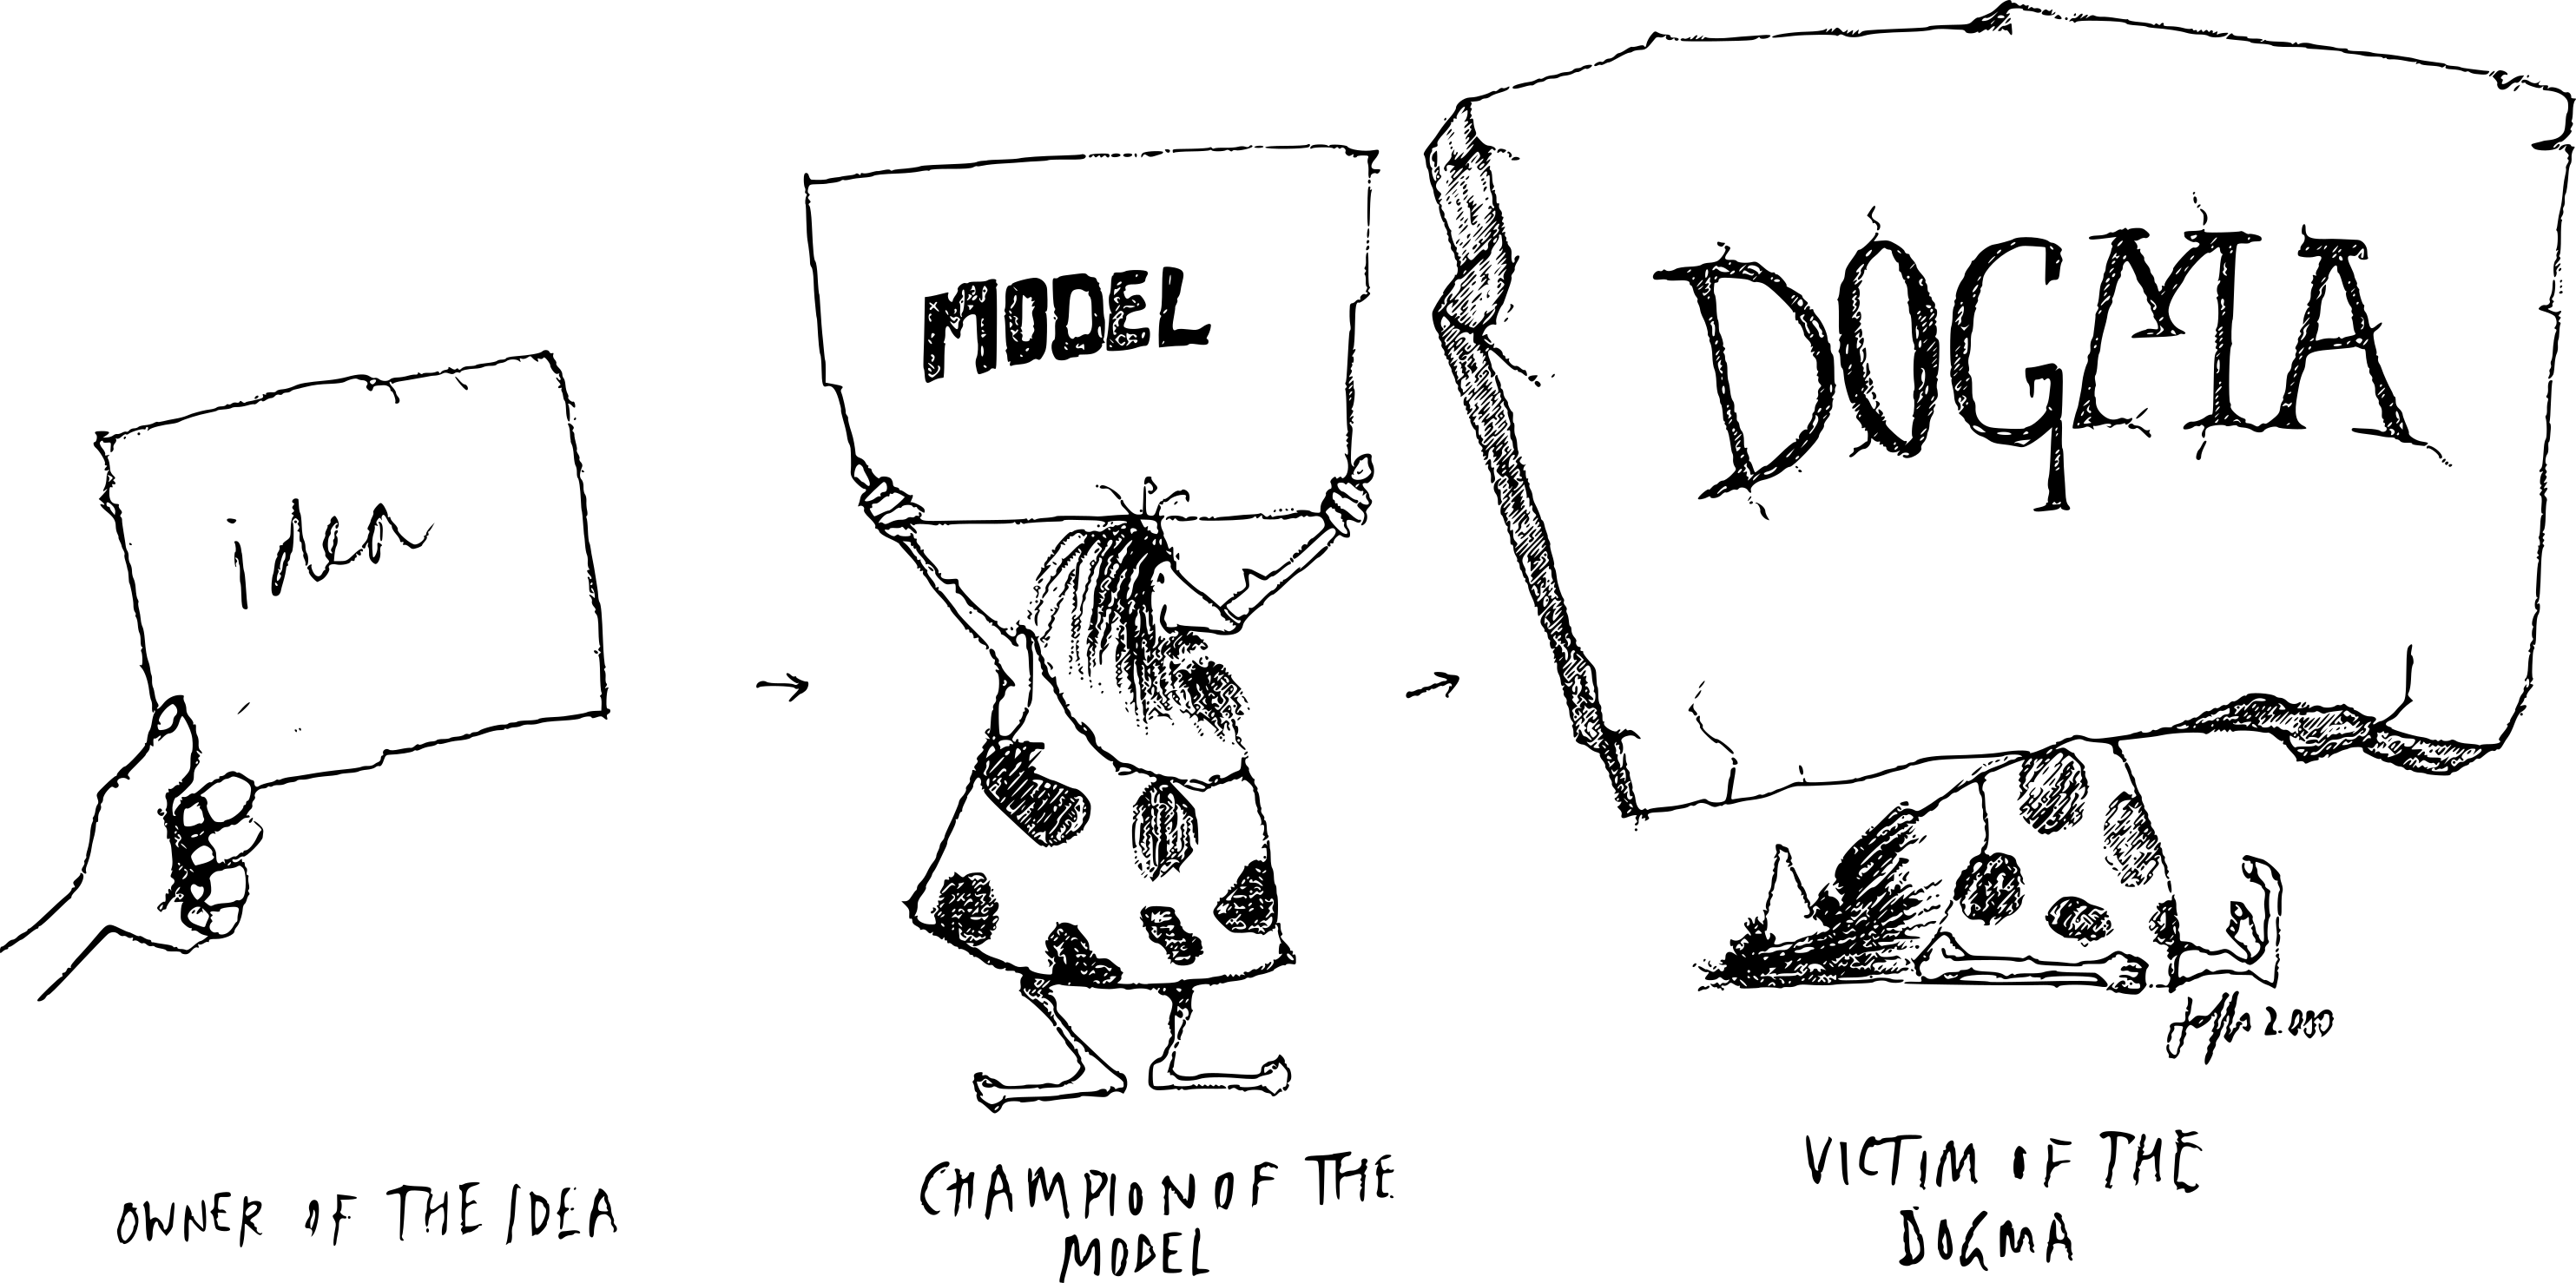
\includegraphics[width=\linewidth]{ch.discussion/imgs/dogma.png}
    \caption{\textbf{The hourglass model as a dogma}. \cite{Caveman2000}}
    \label{fig:dogma}
\end{figure}

\section{scepia: gene regulatory networks}

Almost all gene regulatory approaches are context specific. But in the end a single set of instructions (DNA) for all contexts.

\section{Do I regret seq2science?}

\section{The future of biology}

\subsection{Computational}



\subsection{lack of unified data encode like stuff}

For seq2science paper we tried paper X, Y, Z. DIFFICULT to get similar results.     

% No similarity between replicates:
% https://www.nature.com/articles/s41467-019-12687-4
% 
%  - drosophila sample missing and two other samples swapped
%  - inverse hourglass time orientation has negative values

NCBI sra is growing exponentially \cite{srawebsite}, but it is poorlymaintained.? It is an absolute pain to download from NCBI sra, hence sra-explorer, pysradb, fetchfastq, nf-core/fetchngs, and seq2science download-fastq workflow. Even more painful is that samples are submitted in non-standardized format. Need for MetaSRA and ALE. Works poorly, and is not necessary. Just properly add data. ENCOED is really nice

Single cell datasets often useless as only two out of three reads submitted. Single cell data is increasingly large.

\subsection{Open Science}



\subsection{Too much descriptive, not enough understanding}

\subsection{Move away from mRNA}

mRNA and protein relation.
The correlation between protein expression and mRNA expression seems high (0.87) measured across cell types. However, genes with high protein expression generally have high mRNA expression. So it is easy to get high prediction. If you want to predict a single gene you get correlation of 0.41. Simpson's paradox! 
https://www.nature.com/articles/nature23293

https://www.biorxiv.org/content/10.1101/2023.05.23.541948v1

cool work of michael levine on xenobots

% https://twitter.com/nimwegenlab/status/1671923176626847744?s=12&t=oyB_faiBr8aHqHcjXZE50A

\begin{figure}[H]
    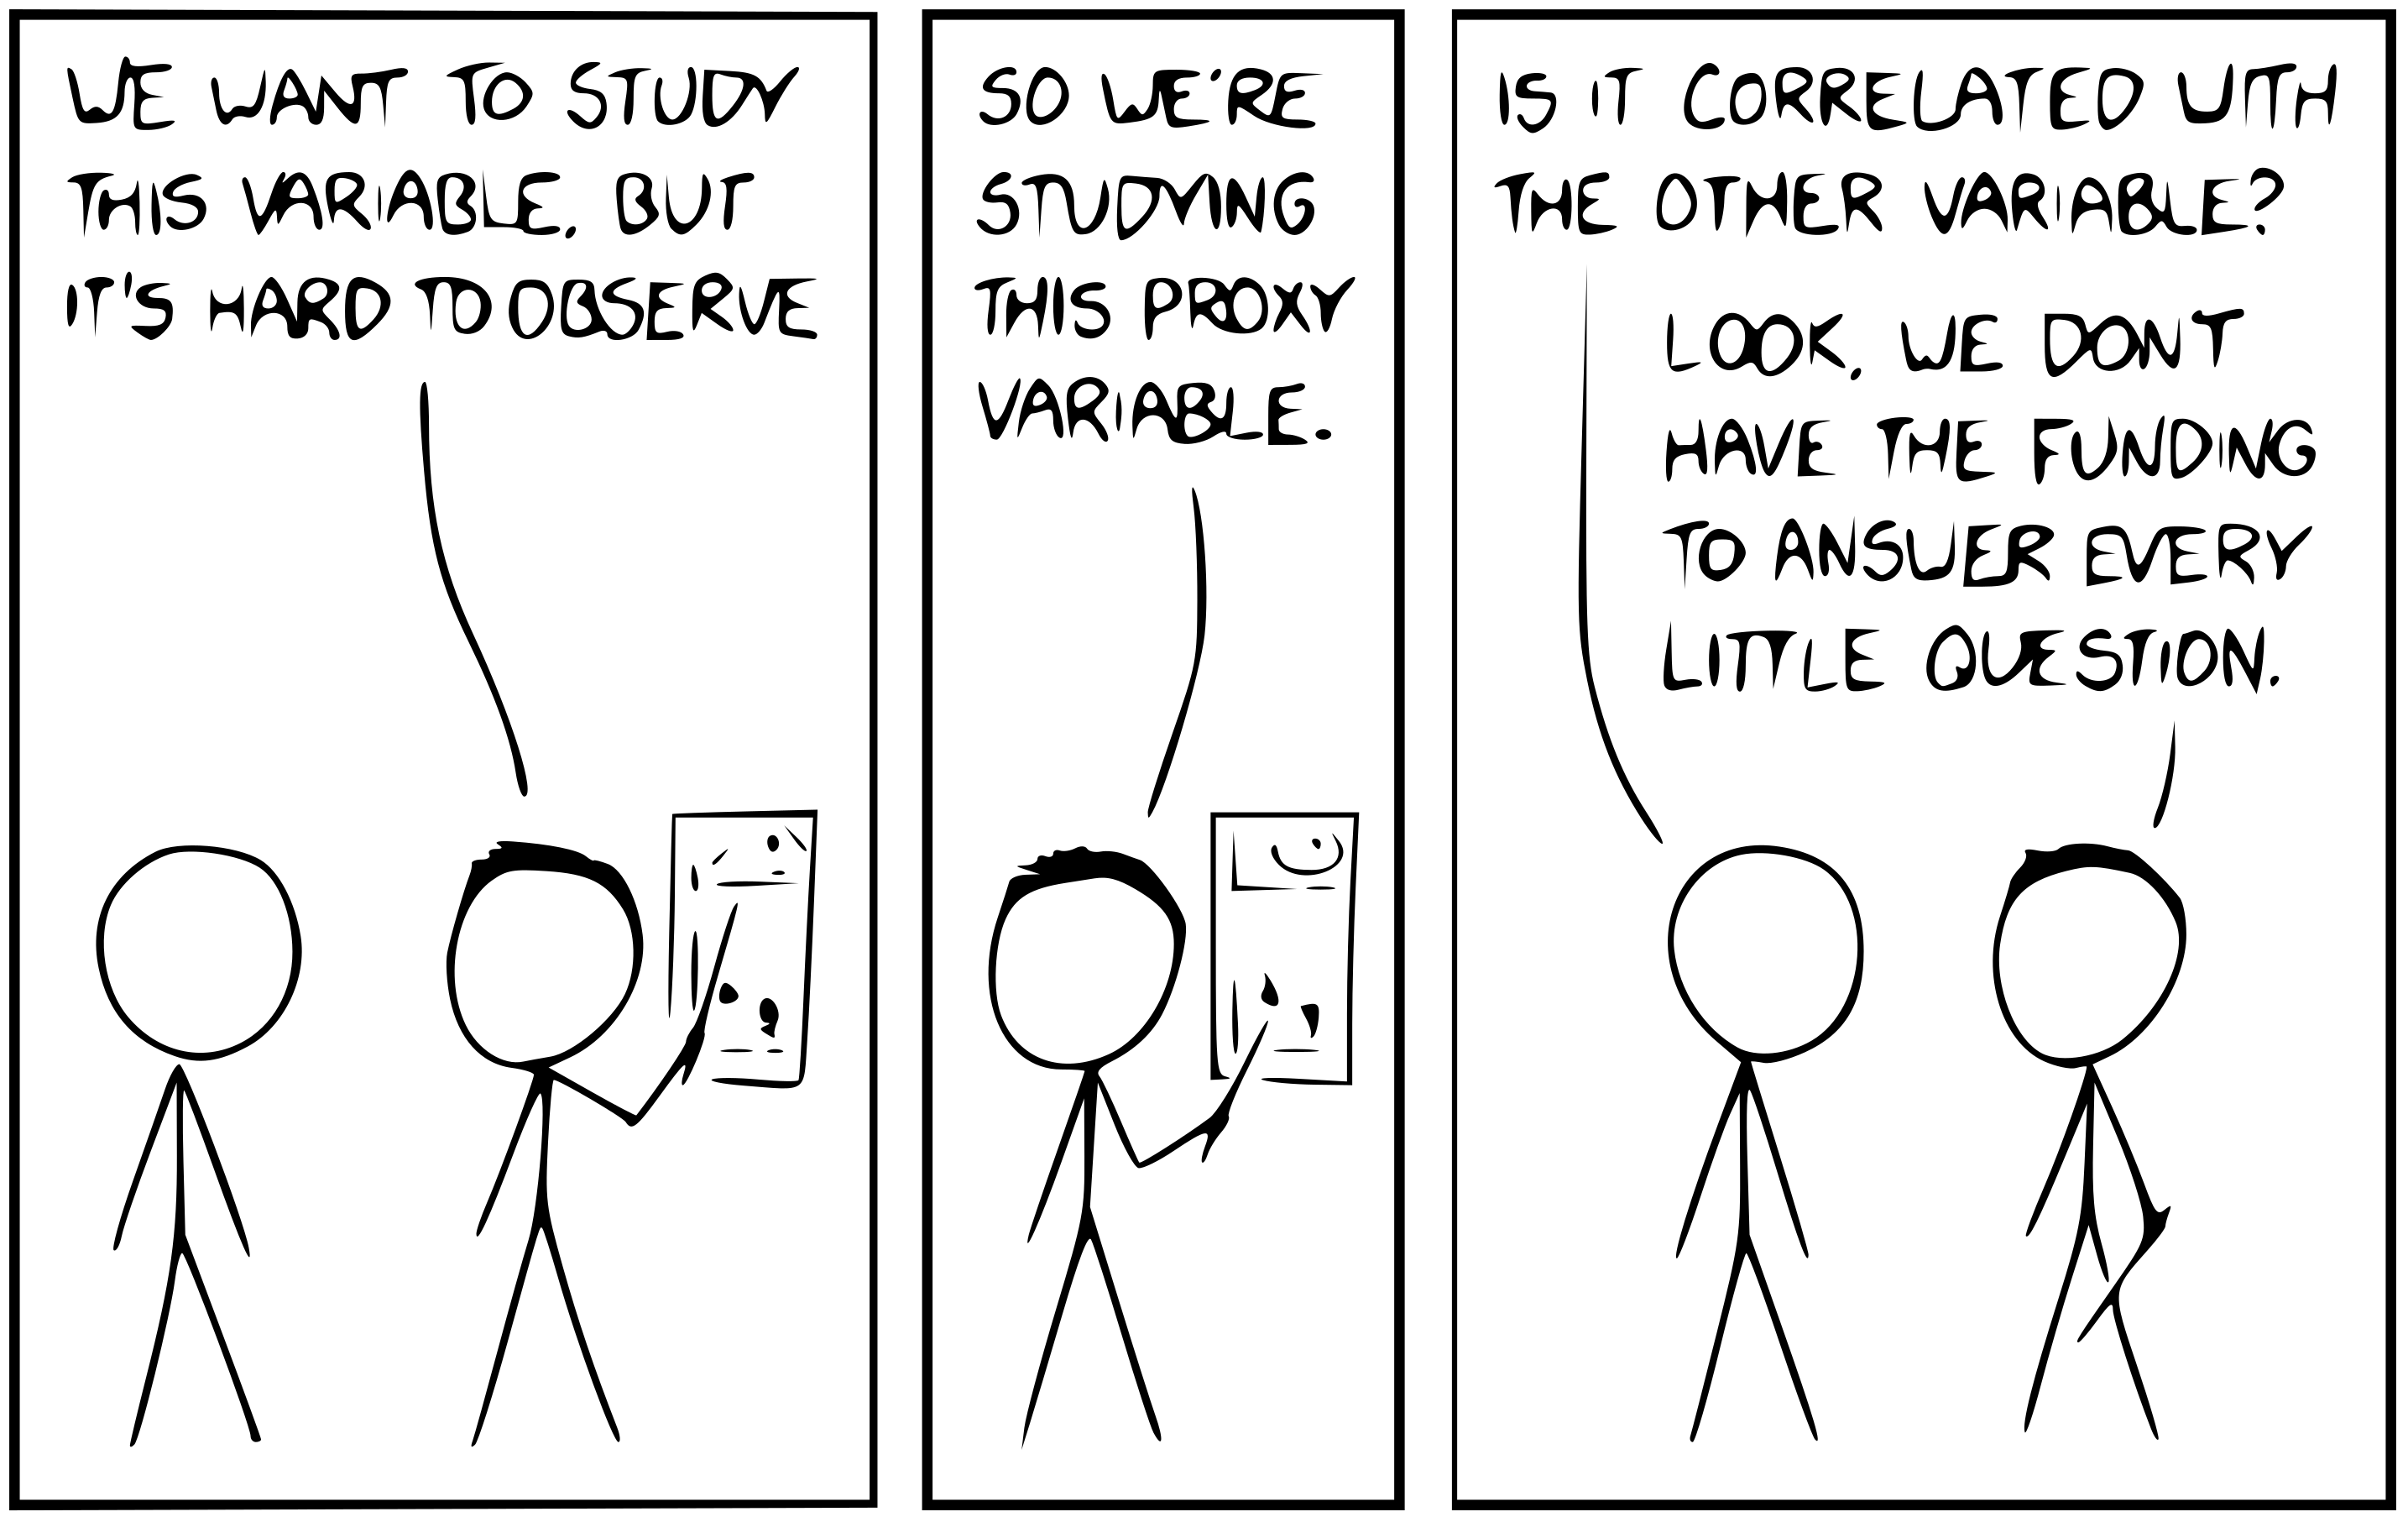
\includegraphics[width=\linewidth]{ch.discussion/imgs/xkcd.png}
    \caption{\textbf{xkcd}. URL: https://xkcd.com/2652}
    \label{fig:xkcd}
\end{figure}

\subsection{Stop blaming "the incentives"}

incentives: https://www.talyarkoni.org/blog/2018/10/02/no-its-not-the-incentives-its-you/

\subsection{Self-correcting}

e.g. wild growth covid papers

papers keep on being cited after retraction or criticism. Number one paper of percentage of genome is functional gives highly criticized ENCODE paper.

highlight cancer genome paper.



% Biology is messy, but that does not mean computational biology has to be.
